\setcounter{ExampleCounter}{1}
We began by calculating the probabilities of single events occurring, and then we learned how to combine events using \emph{OR}.  Now we ask a different question: suppose we know how to calculate the probability of $A$ and the probability of $B$ on their own; how can we calculate the probability that $A$ \emph{AND} $B$ both occur?  To set this up, we'll look at two situations: flipping a coin twice and drawing two cards \emph{without replacement} (this will be important).

\paragraph{Flipping a coin twice} If\marginnote{Independent events:\\ don't affect each other\\ (whether the first flip is heads or tails, the probabilities for the second flip are not impacted)} we flip a coin twice in succession, the sample space is \[S=\{HH, HT, TH, TT\}.\]  Now suppose we ask the following questions:
\begin{enumerate}
\item What is the probability that the first flip results in a head?
\begin{center}
Either by noticing that there are two possibilities for the first flip or by looking at the sample space and seeing that there are two outcomes (out of four total) that correspond to a head on the first flip, we can reason that this probability is 1/2.
\end{center} 
\item What is the probability that the second flip results in a tail?
\begin{center}
Using the same reasoning, we conclude that this probability is also 1/2.
\end{center} 
\item What is the probability that the first flip results in a head \emph{AND} the second flip results in a tail?
\begin{center}
Looking at the sample space, we notice that there is exactly one outcome that corresponds to this (out of four), so this probability is 1/4.
\end{center}
\end{enumerate}

Notice that the probability of both happening together is the probability of one times the probability of the other:
\[\dfrac{1}{2} \cdot \dfrac{1}{2} = \dfrac{1}{4}\]

Seeing this, and noting the title of the section, we may be tempted to jump to the conclusion that the probability of $A$ \emph{AND} $B$ is simply the probability of $A$ times the probability of $B$.  However, the next scenario illustrates that we need to be a bit more careful.

Just as we found with the addition rule, there is a simple version that works if a certain condition is met, and if not, there is a more general version of the multiplication rule.

\paragraph{Drawing two cards without replacement}
Suppose\marginnote{Dependent events:\\ affect each other\\ (after pulling out the first card, the deck has changed, so the probabilities have shifted)} we draw one card, and then \emph{without} placing it back and re-shuffling the deck, we draw a second card.  What is the probability that we draw two Aces?\\

This situation is different from the previous one, because now what happens on the first draw affects the probabilities for the second draw.  In other words, the probability of drawing an Ace the first time is 4/52.  If we draw an Ace the first time, there are only 3 Aces left and 51 total cards left, so the probability of drawing an Ace the second time is 3/51.  However, if we do not draw an Ace the first time, there are still 4 Aces in the deck, so the probability of drawing an Ace the second time is 4/51.  We can illustrate this with a branching tree diagram.

\begin{center}
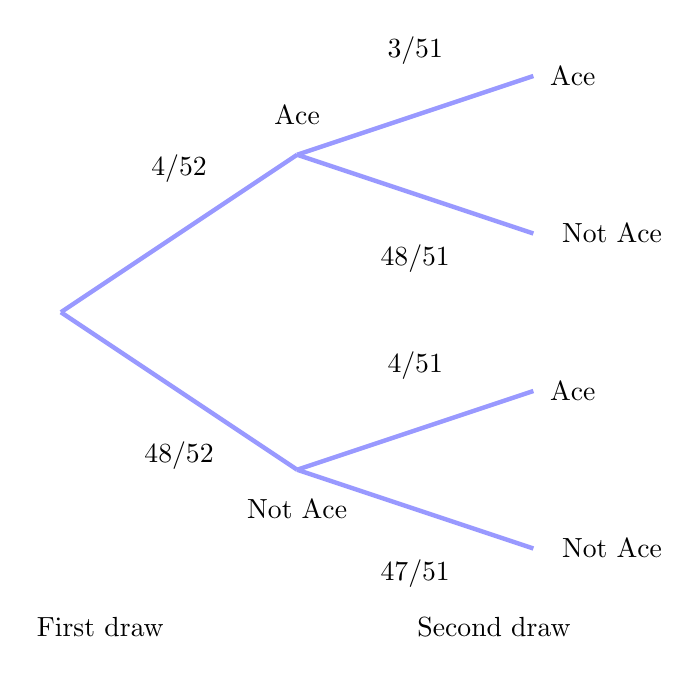
\begin{tikzpicture}
\draw [ultra thick,color=blue!40] (-3,0) -- (0,2) node[midway, above, yshift=0.5cm, color=black] {4/52};
\draw [ultra thick,color=blue!40] (0,2) -- (3,3) node[midway, above, yshift=0.5cm, color=black] {3/51};
\draw [ultra thick,color=blue!40] (0,2) -- (3,1) node[midway, below, yshift=-0.5cm, color=black] {48/51};

\draw [ultra thick,color=blue!40] (-3,0) -- (0,-2) node[midway, below, yshift=-0.5cm, color=black] {48/52};
\draw [ultra thick,color=blue!40] (0,-2) -- (3,-1) node[midway, above, yshift=0.5cm, color=black] {4/51};
\draw [ultra thick,color=blue!40] (0,-2) -- (3,-3) node[midway, below, yshift=-0.5cm, color=black] {47/51};

\draw [yshift=-4cm,xshift=-2.5cm] node {First draw};
\draw [yshift=-4cm,xshift=2.5cm] node {Second draw};
\draw [yshift=2.5cm,xshift=0cm] node {Ace};
\draw [yshift=-2.5cm,xshift=0cm] node {Not Ace};
\draw [yshift=3cm,xshift=3.5cm] node {Ace};
\draw [yshift=1cm,xshift=4cm] node {Not Ace};
\draw [yshift=-1cm,xshift=3.5cm] node {Ace};
\draw [yshift=-3cm,xshift=4cm] node {Not Ace};

\end{tikzpicture}
\end{center}

Now the probability of drawing an Ace both times is the probability of drawing an Ace the first time multiplied by the probability of drawing an Ace the second time \textbf{given that we drew an Ace the first time}.  Notice on the tree diagram that this corresponds to following the upward branch both times.

This is because \emph{only} if we draw an Ace the first time do we have any chance of fulfilling the scenario; if we fail to draw an Ace the first time, it doesn't matter what we do the second time--we've already failed.

Thus, the probability of drawing an Ace both times is 
\begin{center}
$P($Ace the first time$) \cdot P($Ace the second time IF we drew one the first time$)$\\
\text{}\\
$= \dfrac{4}{52} \cdot \dfrac{3}{51} = \dfrac{12}{2652} \approx 0.0045$
\end{center}

This is what we call \emph{conditional probability}, and it's what we have to consider for the general multiplication rule.

\subsection{Independence}
What was the difference between those two scenarios?  Why, in the first one, could we simply multiply the individual probabilities and in the second we had to think about conditional probability?  The answer lies in what we call \textbf{independence}: when flipping the coin, each time we flipped it had no impact on the other times; when we drew the cards without replacement, though, one draw affected the next.  Notice that we made the careful distinction that we drew without replacement; if we had replaced the first card and re-shuffled the deck before drawing again, the two draws would have been independent.

\begin{proc}{Independence}
Two events are independent if the outcome of one has no effect on the probability of the other occurring.
\end{proc}

Note that saying that two events are \emph{independent} is different than saying that two events are \emph{mutually exclusive}.
\begin{itemize}
\item If two events are independent, they have no effect on each other's likelihood of occurring.
\item If two events are mutually exclusive, they cannot occur together, so they do have an effect on each other's likelihood of occurring (namely, making it impossible).
\end{itemize}
\pagebreak

\begin{example}[https://www.youtube.com/watch?v=ul4iYkGHbAE&list=PLfmpjsIzhzts14-9s5QixRje97EI2oeMF&index=19]{Independent events}
Determine whether these events are independent:

\begin{enumerate}[(a)]
\item A fair coin is tossed two times. The two events are $A$ =  first toss is Heads and $B$ =  second toss is Heads.
\begin{center}
The\marginnote{\bfseries Solution} probability that Heads comes up on the second toss is 1/2 regardless of whether or not Heads came up on the first toss, so these events are independent.
\end{center}

\item The two events $A$ =  \emph{It will rain tomorrow in Frederick, MD} and $B$ =  \emph{It will rain tomorrow in Thurmont, MD} 
\begin{center}
These\marginnote{\bfseries Solution} events are not independent because it is more likely that it will rain in Thurmont on days it rains in Frederick.
\end{center} 

\item You draw a red card from a deck, then draw a second card without replacing the first.
\begin{center}
These\marginnote{\bfseries Solution} events are dependent, specifically because the first card is \textit{not replaced}.  After drawing the first card, the deck looks different than it did before.  There are 25 red cards left and 26 black cards left, so the probabilities have shifted.
\end{center}

\item You draw a face card from the deck, then replace it and re-shuffle the deck before drawing a second card.
\begin{center}
Since\marginnote{\bfseries Solution} you reset the deck between draws, the events are independent.
\end{center}
\end{enumerate}
\end{example}

Now we are ready to formally state the rule that we used in the first scenario at the beginning of the section.
\vspace*{-0.1in}

\subsection{The Multiplication Rule for Independent Events}
\begin{formula}{Probabilities of independent events}
If $A$ and $B$ are independent, then the probability of both $A$ and $B$ occurring is
\[  P( A \mbox{ and } B) = P(A) \cdot P(B) \]

We can generalize this to finitely many independent events $A_1, A_2, \dots, A_k$
\[ P( A_1 \mbox{ and } A_2 \mbox{ and } \dots \mbox{ and } A_k ) = P(A_1) \cdot P(A_2) \cdot ... \cdot P(A_k)  \]

\end{formula}

\begin{example}[https://www.youtube.com/watch?v=twQYgbDkgro&list=PLfmpjsIzhzts14-9s5QixRje97EI2oeMF&index=20]{Coins and dice}
Suppose you flip a coin and roll a six-sided die once. What is the probability you get Tails and an even number?  

\sol
Flipping a coin and rolling a die are independent events, since the outcome of one does not effect the outcome of the other. Thus, we compute it as follows:
\begin{align*}
P(T \mbox{ and } \mbox{\emph{even number}}) &= P(T) \cdot P(\mbox{\emph{even number}})\\
&= \frac{1}{2} \cdot \frac{3}{6}\\
&= \frac{3}{12} = \boxed{\frac{1}{4} = 0.25}
\end{align*}
\end{example}

\begin{try}[http://hartleymath.com/versatilemath/tryit/\#/probability--drawing-a-king-and-black-card]
Assume you have a 52 card deck, and you select two cards at random. Also
assume that you replace and reshuffle after each selection. Find the probability of drawing a king first and then a black card.
\end{try}

\begin{example}[https://www.youtube.com/watch?v=GL_EhwQq-98&list=PLfmpjsIzhzts14-9s5QixRje97EI2oeMF&index=21]{Left-handed population}
About 9\% of people are left-handed. Suppose 2 people are selected at random from the U.S. population. Because\marginnote{Unlike a deck of cards, in which removing one card makes a noticeable difference, removing one person from hundreds of millions makes such a small difference that we can ignore it for simplicity.} the sample size of 2 is
very small relative to the population, it is reasonable to assume these two people are independent. What is the probability that both are left-handed? 

\solline
The probability the first person is left-handed is 0.09, which is the same for the second person: \[P(\textrm{both left}) = 0.09 \cdot 0.09  = \boxed{0.0081} \]
\end{example}

\begin{try}[http://hartleymath.com/versatilemath/tryit/\#/probability--commuting-in-the-same-type-of-vehicle]
According to the US Census, in 2009 86.1\% of working adults commuted in a car, truck, or van. If three people are selected from the population of working adults, what is the probability that all three commuted in a car, truck, or van?
\end{try}

\begin{example}[https://www.youtube.com/watch?v=670VxNZAcP8&list=PLfmpjsIzhzts14-9s5QixRje97EI2oeMF&index=22]{Boys and girls}
Assuming that probability of having a boy is 0.5, find the probability of a family that has 3 children having 3 boys. 

\sol
Since the gender of each child is independent, we use the multiplication formula for independent events:
\begin{align*}
P(\mbox{3 } boys ) &= P(boy) \cdot P(boy) \cdot P(boy)\\
&= 0.5 \cdot 0.5 \cdot 0.5 = \boxed{0.125}
\end{align*}
\end{example}

\begin{try}[http://hartleymath.com/versatilemath/tryit/\#/probability--colors-of-socks-and-shirt]
In your drawer you have 10 pairs of socks, 6 of which are white, and 7 tee shirts, 3 of which are white. If you randomly reach in and pull out a pair of socks and a tee shirt, what is the probability that both are white?
\end{try}

\subsection{The Multiplication Rule for Dependent Events}
In the second scenario at the beginning of the section, where the events were not independent, we found that we could calculate the probability of both happening by multiplying the probability of the first by the probability that the second occurred IF the first had happened.  We call this \textbf{conditional probability}: the probability that $B$ happens on the \emph{condition} that $A$ already happened.

The notation we use is \[P(B | A).\]
For example, in the scenario where we wanted to draw two Aces in a row, we could write the conditional probability for the second draw as 
\begin{center}
$P($ace on second draw $|$ ace on first draw$)$
\end{center}

The vertical bar | is read as ``given,'' so the above expression is short for ``The probability that an ace is drawn on the second draw given that an ace was drawn on the first draw.'' 
\pagebreak

As we noted earlier, after an ace is drawn on the first draw, there are 3 aces out of 51 total cards left. This means that the conditional probability of drawing an ace after one ace has already been drawn is $3/51 = 1/17$. Thus, the probability of both cards being aces is
\[ \frac{4}{52} \cdot \frac{3}{51} = \frac{12}{2652} = \frac{1}{221} \]

\begin{formula}{Multiplication formula for dependent events}
If events $A$ and $B$ are not independent, then
\[  P(A \mbox{ and } B) = P(A) \cdot  P(B |A ) \]
\end{formula} 

Note that this, like with the addition rule, is the general multiplication rule; if $A$ and $B$ are independent, $P(B|A)=P(B)$ (because the probability of $B$ is the same regardless of whether $A$ has occurred or not) and the general multiplication formula becomes the simpler form for independent events that we have already seen.

\begin{example}[https://www.youtube.com/watch?v=6CvJ2GJ6HHU&list=PLfmpjsIzhzts14-9s5QixRje97EI2oeMF&index=23]{Drawing cards without replacement}
If you pull 2 cards out of a deck, what is the probability that both are spades? 

\sol
The probability that the first card is a spade is $13/52$, while the probability that the second card is a spade, given the first was a spade, is $12/51$. Thus, the probability that both cards are spades is
\begin{align*}
P(\mbox{2 } spades) &= \frac{13}{52} \cdot \frac{12}{51}\\
&= \boxed{\frac{156}{2652} \approx 0.0588}
\end{align*}
\end{example}

\begin{try}[http://hartleymath.com/versatilemath/tryit/\#/probability--two-pairs-of-white-socks]
In your drawer you have 10 pairs of socks, 6 of which are white. If you reach in and
randomly grab two pairs of socks, what is the probability that both are white?
\end{try}

\begin{example}[https://www.youtube.com/watch?v=j8BFTGwza9s&list=PLfmpjsIzhzts14-9s5QixRje97EI2oeMF&index=24]{M\&M's}

A bag of M\&M's contains the following breakdown of colors:

\begin{center}
\begin{tabular}{c c c c c c}
\textbf{Red} & \textbf{Yellow} &  \textbf{Brown} & \textbf{Blue} & \textbf{Orange} & \textbf{Green} \\ \hline
& & & & & \\
12 & 18 & 24 &  22 &  13 & 17 \\
\end{tabular}
\end{center}
Suppose you pull two M\&M's out of the bag (without replacing the candy after each pull). Find the following probabilities:
\begin{enumerate}[(a)]
\item The probability of drawing two red candies
\item The probability of drawing a blue candy and then a brown candy, in that order
\item The probability of \textbf{not} drawing two green candies
\item The probability of drawing one orange candy and one yellow candy (note that order is not mentioned)
\end{enumerate}
\pagebreak

\sol
\begin{enumerate}[(a)]
\item Since there are a total of 106 candies at first, the probability of drawing a red candy on the first try is 12/106.  Assuming that first try is successful, there will be a total of 105 candies left, of which 11 are red, so the probability of drawing a red candy on the second try will be 11/105:
\begin{align*}
P(red,\ red) &= P(red) \cdot P(red\ |\ red)\\
&= \frac{12}{106} \cdot \frac{11}{105}\\
&= \boxed{\frac{132}{11,130} \approx 0.0119}
\end{align*}

\item At first, there will be 22 blue candies out of a total of 106, and if the first try yields a blue one, all the brown ones (24) will still be in the bag, which will then contain 105 in total:
\begin{align*}
P(blue,\ brown) &= P(blue) \cdot P(brown \ | \ blue)\\
&= \frac{22}{106} \cdot \frac{24}{105}\\
&= \boxed{\frac{528}{11,130} \approx 0.0474}
\end{align*}

\item In order to \emph{not} draw two green candies, we could start thinking of all the possible combinations \emph{other} than \emph{green, green}, but it's much easier to use the complement rule.  We can calculate the probability of drawing two green candies the same way we did at the beginning with red candies, then subtract this answer from 1:
\begin{align*}
P(not\ 2\ green) &= 1-P(2 \ green)\\
&= 1 - P(green) \cdot P(green \ | \ green)\\
&= 1-\frac{17}{106} \cdot \frac{16}{105}\\
&= 1 - \frac{272}{11,130}\\
&= \boxed{\dfrac{10,858}{11,130} \approx 0.9756}
\end{align*}

This is important: it is much easier to calculate the probability of drawing two green candies first, and then subtracting this from one.  If we didn't do this, we would have to calculate three separate probabilities and add them together:
\begin{itemize}
\item Drawing\marginnote{$(17/106) \cdot (89/105)$} a green, then a non-green candy
\item Drawing\marginnote{$(89/106) \cdot (17/105)$} a non-green, then a green candy
\item Drawing\marginnote{$(89/106) \cdot (88/105)$} a non-green, then a non-green candy
\end{itemize}
%This is one reason that we need the complement rule, because it makes probabilities like these easier to calculate.

\item This time, order is not significant, so there are two possibilities:
\begin{itemize}
\item Draw orange, then yellow
\item Draw yellow, then orange
\end{itemize}
Since these two outcomes are mutually exclusive, the final answer will be the sum of these two.  To calculate each individual answer, we can use the same approach we used with the blue and brown example:
\begin{align*}
P(orange\ and\ yellow) &= P(orange,\ yellow) + P(yellow,\ orange)\\
&= P(orange) \cdot P(yellow\ |\ orange)\\
&\ \ + P(yellow) \cdot P(orange\ |\ yellow)\\
&= \dfrac{13}{106} \cdot \dfrac{18}{105} + \dfrac{18}{106} \cdot \dfrac{13}{105} = \dfrac{234}{11,130} + \dfrac{234}{11,130}\\
&= \boxed{\dfrac{468}{11,130} \approx 0.0420}
\end{align*}
Notice that the answer for each part was the same, so we could also have simply calculated the probability of one ordering, then doubled the answer.
\end{enumerate}
\end{example}
\vfill
\pagebreak

It is often useful to be able to calculate conditional probabilities using contingency tables, so let's take a look at an example of that.

The key here is that when we encounter the word \emph{given}, it means that we will restrict ourselves only to that category, meaning that the denominator will not be the total number of observations, but rather the total for the relevant row or column.

\begin{example}[https://www.youtube.com/watch?v=0oCoc5B1lVU&list=PLfmpjsIzhzts14-9s5QixRje97EI2oeMF&index=25]{Conditional Probability and Contingency Tables}
We will again use the data regarding 130 FCC students, broken down by gender and dominant hand:
\begin{center}
\begin{tabular}{l | c c | c}
\textbf{Gender} & \textbf{Right-handed} & \textbf{Left-handed} & \textbf{Total} \\ \hline 
\textbf{Female} & 58 & 13 & 71\\
\textbf{Male} & 47 & 12 & 59  \\ \hline
\textbf{Total} & 105 & 25 & 130 \\ 
\end{tabular}
\end{center}
\begin{enumerate}[(a)]
\item What is the probability that a randomly chosen student is female, given that the student is left-handed?
\item What is the probability that a randomly chosen student is right-handed, given that the student is male?
\end{enumerate}

\sol
\begin{enumerate}
\item To calculate conditional probabilities from a contingency table, all we have to do is restrict ourselves to the ``given'' category.  For this one, we are given that the student is left-handed, so we'll only look at the left-handed column and see what proportion of those are female.  The total number of left-handed students is 25, and within that group, 13 are female and 12 are male:
\[P(female \ | \ left) = \boxed{\frac{13}{25} = 0.52}\]

\item Here we'll only look at the male row, since we're given that the randomly chosen student is male.  All we need to calculate is what proportion of males in this group are right-handed:
\[P(right \ | \ male) = \boxed{\frac{47}{59} \approx 0.7966}\]
\end{enumerate}
\end{example}

We'll wrap up this section with a short discussion of a surprising application of conditional probability: medical tests.\\

Let's say, for instance, that a certain disease infects 100 out of 100,000 people.  There is a test for this disease, and it is correct 99\% of the time.  Now, here's the question: if you go to the doctor and take this test, and the result is positive (meaning the test says that yes, you have the disease), how likely is it that you truly have it?\\

The intuitive answer is that it must be 99\% likely that you have the disease, since the test is correct 99\% of the time.  However, the truth is more complicated.

The key to this problem is that the disease is fairly rare.  So when a test comes back positive, there are two possibilities: either you have the disease or the test is wrong.  Notice that there is only a 1 in 1000 chance that you have the disease, while there is a 1 in 100 chance that the test is wrong.  Therefore, it turns out that \emph{even with a positive result, you are more likely to be healthy}.  Of course, this ignores the fact that you may have only gotten the test because you were showing symptoms, in which case the odds of having the disease would be much higher than 1 in 1000.

To get a more precise answer, we can build a contingency table like the one in the last example.  Let's start with a group of 100,000 people: 100 of them are sick and 99,900 are healthy.
\begin{center}
\begin{tabular}{l | c c | c}
& \textbf{Sick} & \textbf{Healthy} & \textbf{Total}\\ \hline
\textbf{Positive Test} & & & \\
\textbf{Negative Test} & & & \\ \hline
\textbf{Total} & 100 & 99,900 & 100,000
\end{tabular}
\end{center}
\pagebreak

Now, let's imagine giving everyone in this group a test (remember, the test is correct 99\% of the time and wrong 1\% of the time).  In the sick group, how many would test positive and how many would test negative?  Since the correct result for this group is a positive test, 99 of them would get a positive result and 1 would get a negative result.
\begin{center}
\begin{tabular}{l | c c | c}
& \textbf{Sick} & \textbf{Healthy} & \textbf{Total}\\ \hline
\textbf{Positive Test} & 99 & & \\
\textbf{Negative Test} & 1 & & \\ \hline
\textbf{Total} & 100 & 99,900 & 100,000
\end{tabular}
\end{center}

What about the healthy group?  For them, a positive test is the wrong result, so 1\% of them (999 people) would see that, while the remainder would get a correct negative result.
\begin{center}
\begin{tabular}{l | c c | c}
& \textbf{Sick} & \textbf{Healthy} & \textbf{Total}\\ \hline
\textbf{Positive Test} & 99 & 999 & 1098\\
\textbf{Negative Test} & 1 & 98,901 & 98,902\\ \hline
\textbf{Total} & 100 & 99,900 & 100,000
\end{tabular}
\end{center}

Now that we've filled out all the possibilities, we can return to the question: suppose you get a positive result; what's the probability that you're sick?  We can state this more precisely using conditional probability: what is the probability that you are sick, \emph{given} that you have a positive test?\\

Using the approach of the last example, we can do this by focusing on the row that shows everyone with a positive test, and out of that group, find the probability of being sick:
\[P(sick\ |\ positive\ result) = \dfrac{99}{1098} \approx 0.09\]

There's only about a 9\% chance that you are sick, \emph{even after getting a positive test}.  Again, the reason for this is that this disease is \emph{known} to be rare, while an incorrect test result is not as rare.\\

\begin{comment}
We can use a little algebra to write that last line in general form: since
\[P(A \textrm{ and } B) = P(A) \cdot P(B\ |\ A),\]
we can rewrite this by solving for the conditional probability (divide both sides by $P(A)$).

\begin{formula}{Conditional Probability}
Conditional probability can be calculated as follows, if $P(A \textrm{ and } B)$ and $P(A)$ are both known:
\[P(B\ |\ A) = \dfrac{P(A \textrm{ and } B)}{P(A)}\]
\end{formula}

In the example of the medical test, it looks like
\[P(sick\ |\ positive\ result) = \dfrac{P(sick \textrm{ and } positive\ result)}{P(positive\ result)}\]
and, of course, these probabilities can be found on the contingency table as well.
\end{comment}